\documentclass[12pt,a4paper]{article}

% ─── Page Layout ───────────────────────────────────────────────────────────────
\usepackage[a4paper, margin=0.8in, headheight=14pt]{geometry}

% ─── Fonts (XeLaTeX) ───────────────────────────────────────────────────────────
\usepackage{fontspec}
\usepackage{unicode-math}
\setmainfont{TeX Gyre Pagella}
\setmonofont[Scale=0.88]{TeX Gyre Cursor}
\setmathfont{Latin Modern Math}

% ─── Packages ──────────────────────────────────────────────────────────────────
\usepackage{xcolor}
\usepackage{colortbl}
\usepackage{titlesec}
\usepackage{enumitem}
\usepackage{tabularx}
\usepackage{booktabs}
\usepackage{array}
\usepackage{amsmath}
\usepackage{tikz}
\usetikzlibrary{shapes.geometric, arrows.meta, positioning, calc, fit, decorations.pathreplacing}
\usepackage{tcolorbox}
\tcbuselibrary{skins, breakable}
\usepackage{hyperref}
\usepackage{fancyhdr}
\usepackage{graphicx}
\usepackage{microtype}
\hyphenpenalty=10000
\exhyphenpenalty=10000
\sloppy
\usepackage{caption}
\usepackage{setspace}
\usepackage{multirow}
\usepackage{tocloft}

% ─── Q&A helper ────────────────────────────────────────────────────────────────
\newcommand{\Q}[1]{\textbf{#1}\par\noindent\ignorespaces}

% ─── Colour Palette ────────────────────────────────────────────────────────────
\definecolor{myred}{RGB}{196,30,58}
\definecolor{mydark}{RGB}{30,30,50}
\definecolor{mygreen}{RGB}{14,120,80}
\definecolor{myteal}{RGB}{0,130,140}
\definecolor{myamber}{RGB}{180,100,0}
\definecolor{mypurple}{RGB}{100,30,160}
\definecolor{mygray}{RGB}{246,247,249}
\definecolor{mgframe}{RGB}{180,185,200}
\definecolor{watermark}{RGB}{145,150,170}
\definecolor{hdrred}{RGB}{250,232,235}
\definecolor{hdrgreen}{RGB}{220,244,233}
\definecolor{hdrteal}{RGB}{220,242,244}
\definecolor{hdramber}{RGB}{253,242,215}
\definecolor{hdrpurple}{RGB}{238,228,255}
\definecolor{hdrgray}{RGB}{238,240,245}
\definecolor{rowalt}{RGB}{250,251,253}

% ─── Section Formatting ────────────────────────────────────────────────────────
\titleformat{\section}
  {\large\bfseries\color{myred}}{\thesection.}{0.5em}{}
  [\vspace{1pt}{\color{myred}\rule{\linewidth}{0.8pt}}]
\titleformat{\subsection}
  {\normalsize\bfseries\color{myteal}}{\thesubsection}{0.5em}{}
\titlespacing*{\section}{0pt}{18pt}{7pt}
\titlespacing*{\subsection}{0pt}{11pt}{4pt}

% ─── Paragraph ─────────────────────────────────────────────────────────────────
\setlength{\parindent}{0pt}
\setlength{\parskip}{4pt}

% ─── TOC Styling ───────────────────────────────────────────────────────────────
\renewcommand{\cfttoctitlefont}{\large\bfseries\color{myred}}
\renewcommand{\cftaftertoctitle}{\par\noindent{\color{myred}\rule{\linewidth}{0.8pt}}}
\setlength{\cftbeforetoctitleskip}{0pt}
\setlength{\cftaftertoctitleskip}{6pt}
\renewcommand{\cftsecfont}{\normalsize\bfseries\color{mydark}}
\renewcommand{\cftsecpagefont}{\normalsize\bfseries\color{mydark}}
\renewcommand{\cftsecleader}{\cftdotfill{\cftdotsep}}
\setlength{\cftbeforesecskip}{7pt}
\renewcommand{\cftsubsecfont}{\small\color{mydark}}
\renewcommand{\cftsubsecpagefont}{\small\color{mydark}}
\setlength{\cftbeforesubsecskip}{3pt}
\setlength{\cftsubsecindent}{1.4em}

% ─── Table helpers ─────────────────────────────────────────────────────────────
\renewcommand{\arraystretch}{1.45}
\setlength{\tabcolsep}{6pt}
\arrayrulecolor{mydark}
\newcolumntype{B}[1]{>{\small\bfseries\raggedright\arraybackslash}m{#1}}
\newcolumntype{Y}{>{\small\raggedright\arraybackslash}X}
\renewcommand{\tabularxcolumn}[1]{m{#1}}

% ─── Header / Footer ───────────────────────────────────────────────────────────
\pagestyle{fancy}
\fancyhf{}
\fancyhead[L]{\small\color{myred}\textbf{PE-EC701C}\;\color{mydark}--- Mobile Communication and Networks}
\fancyhead[R]{\small\color{myteal}\textbf{Module 3 Notes}}
\fancyfoot[C]{\small\color{mydark}\thepage}
\fancyfoot[R]{\small\color{watermark}\textit{\copyright\ Biraj}}
\renewcommand{\headrulewidth}{0.5pt}
\renewcommand{\footrulewidth}{0.3pt}

% ─── Hyperref ──────────────────────────────────────────────────────────────────
\hypersetup{
  colorlinks=true, linkcolor=myteal, urlcolor=myteal,
  pdfauthor={Biraj Sarkar},
  pdftitle={PE-EC701C --- Module 3 Notes}
}

% ─── tcolorbox styles ──────────────────────────────────────────────────────────
\tcbset{
  tikzbox/.style={
    colback=mygray, colframe=mgframe, boxrule=0.6pt, arc=4pt,
    left=8pt, right=8pt, top=6pt, bottom=6pt,
    colbacktitle=mgframe, coltitle=mydark,
    fonttitle=\small\bfseries
  },
  defbox/.style={
    colback=hdrgreen, colframe=mygreen, boxrule=0.8pt, arc=4pt,
    left=9pt, right=9pt, top=6pt, bottom=6pt,
    colbacktitle=mygreen, coltitle=white,
    fonttitle=\small\bfseries
  },
  formulabox/.style={
    colback=hdrteal, colframe=myteal, boxrule=0.8pt, arc=4pt,
    left=9pt, right=9pt, top=7pt, bottom=7pt,
    colbacktitle=myteal, coltitle=white,
    fonttitle=\small\bfseries
  },
  examplebox/.style={
    colback=hdramber, colframe=myamber, boxrule=0.8pt, arc=4pt,
    left=9pt, right=9pt, top=6pt, bottom=6pt,
    colbacktitle=myamber, coltitle=white,
    fonttitle=\small\bfseries
  },
  masonbox/.style={
    colback=hdrpurple, colframe=mypurple, boxrule=0.8pt, arc=4pt,
    left=9pt, right=9pt, top=6pt, bottom=6pt,
    colbacktitle=mypurple, coltitle=white,
    fonttitle=\small\bfseries
  },
  exambox/.style={
    colback=hdrpurple, colframe=mypurple, boxrule=1pt, arc=5pt,
    left=10pt, right=10pt, top=8pt, bottom=8pt,
    colbacktitle=mypurple, coltitle=white,
    fonttitle=\bfseries,
    breakable, title after break={\textbf{Frequently Asked / Viva Questions (contd.)}}}
}
\tcbset{breakable}

% ─── TikZ styles ───────────────────────────────────────────────────────────────
\tikzset{
  block/.style={rectangle, draw=myteal, fill=hdrteal,
    text width=2.4cm, align=center, minimum height=0.95cm,
    font=\small, rounded corners=3pt, line width=0.7pt},
  redblock/.style={rectangle, draw=myred, fill=hdrred,
    text width=2.4cm, align=center, minimum height=0.95cm,
    font=\small, rounded corners=3pt, line width=0.7pt},
  netnode/.style={rectangle, draw=myteal, fill=hdrteal,
    text width=1.5cm, align=center, minimum height=0.8cm,
    font=\small, rounded corners=3pt, line width=0.7pt},
  sumjunc/.style={circle, draw=myamber, fill=hdramber,
    minimum size=0.62cm, font=\small, line width=0.8pt},
  snode/.style={circle, draw=mypurple, fill=hdrpurple,
    minimum size=0.55cm, font=\footnotesize, line width=0.7pt},
  arrow/.style={-Stealth, thick, color=mydark},
  redarrow/.style={-Stealth, thick, color=myred},
  line/.style={thick, color=mydark}
}

% ═══════════════════════════════════════════════════════════════════════════════
\begin{document}
% ═══════════════════════════════════════════════════════════════════════════════

\begin{center}
  {\LARGE\bfseries\color{myred} PE-EC701C --- Mobile Communication and Networks}\\[5pt]
  {\normalsize\color{mydark} Semester VII \quad$\bullet$\quad 3L:0T:0P \quad$\bullet$\quad 3 Credits}\\[3pt]
  {\normalsize\color{myteal}\textbf{Module 3 Exam Notes: Channel Capacity and Mobile Antennas}}\\[3pt]
  {\small\color{mydark} CGEC \;$|$\; B.Tech ECE (2023--27) \;$|$\; \textit{Biraj Sarkar}}
\end{center}
\noindent{\color{myred}\rule{\linewidth}{1.5pt}}
\vspace{2pt}

\hypersetup{linkcolor=mydark}
\tableofcontents
\hypersetup{linkcolor=myteal}
\newpage

% ===============================================================================
\section{Capacity of Wireless Fading Channels}
% ===============================================================================

Channel capacity defines the maximum error-free transmission rate achievable over a communication link. Fading causes the signal-to-noise ratio (SNR) at the receiver to fluctuate, making capacity calculations more complex than in static additive white Gaussian noise (AWGN) channels.

\subsection{Capacity of Flat Fading Channels}
In flat fading channels, the channel gain is constant across the signal bandwidth but varies over time. Let $B$ be the bandwidth, $g(t)$ be the time-varying channel power gain, $P$ be the transmit power, and $N_0$ be the noise PSD. The instantaneous SNR is:
\begin{equation}
  \gamma(t) = \frac{P \cdot g(t)}{N_0 B}
\end{equation}
The capacity depends on what Channel State Information (CSI) is available at the transmitter and receiver:

\begin{enumerate}[label=\textbf{\arabic*.}, leftmargin=*, itemsep=3.5pt]
  \item \textbf{CSI Known at Receiver Only (CSIR):} The transmitter sends data at a constant rate. The average achievable rate over time is the \textbf{Ergodic Capacity}:
    \begin{equation}
      C_{\text{ergodic}} = B \cdot \mathbb{E}\left[ \log_2(1 + \gamma) \right] = B \int_{0}^{\infty} \log_2(1 + \gamma) p(\gamma) \, d\gamma
    \end{equation}
    Where $p(\gamma)$ is the PDF of the SNR (e.g., exponential for Rayleigh fading).
  \item \textbf{CSI Known at Transmitter and Receiver (CSIT + CSIR):} The transmitter dynamically adapts its transmit power $P(\gamma)$ and data rate to match the channel state:
    \begin{equation}
      C = \max_{P(\gamma): \mathbb{E}[P(\gamma)] \le P} B \cdot \mathbb{E}\left[ \log_2\left(1 + \frac{P(\gamma)\gamma}{P}\right) \right]
    \end{equation}
    The optimal power allocation is achieved using the \textbf{water-filling algorithm}.
  \item \textbf{Outage Capacity:} If the channel changes slowly, we cannot guarantee error-free transmission at a constant rate. Outage capacity is defined as the maximum rate $C_{\text{out}}$ that can be supported with a probability of outage less than $\epsilon$:
    \begin{equation}
      P(\text{Capacity} < C_{\text{out}}) = \epsilon
    \end{equation}
\end{enumerate}

\subsection{Capacity of Frequency Selective Channels and Water-Filling}
In frequency selective fading, the channel bandwidth is larger than the coherence bandwidth ($B_s > B_c$). The channel is modeled as a set of parallel independent flat-fading subchannels (or subcarriers) using Orthogonal Frequency Division Multiplexing (OFDM).

\begin{tcolorbox}[defbox]
\textbf{Water-Filling (Water-Pouring) Algorithm:} An optimization algorithm that allocates transmit power across parallel independent communication channels to maximize total capacity under a total power constraint. It allocates more power to channels with high gains (low noise) and zero power to channels with gains below a threshold.
\end{tcolorbox}

Let the bandwidth $B$ be divided into $N$ narrow subchannels, each of width $\Delta f = B/N$. Let $\gamma_i = g_i / (N_0 \Delta f)$ be the normalized channel gain of the $i$-th subchannel. The capacity optimization problem is:
\begin{equation}
  \max_{P_i} \sum_{i=1}^{N} \Delta f \log_2\left(1 + \frac{P_i \cdot g_i}{N_0 \Delta f}\right) \quad \text{subject to } \sum_{i=1}^{N} P_i = P_{\text{total}}, \; P_i \ge 0
\end{equation}
Using Lagrange multipliers, the optimal power allocation for subchannel $i$ is:
\begin{equation}
  P_i = \left( \frac{1}{\lambda_0} - \frac{N_0 \Delta f}{g_i} \right)^{\!+}
\end{equation}
Where $\frac{1}{\lambda_0}$ is the common "water-level" and $(x)^+ = \max(x, 0)$.

\begin{tcolorbox}[tikzbox, title={Water-Filling Algorithm Concept}]
\centering
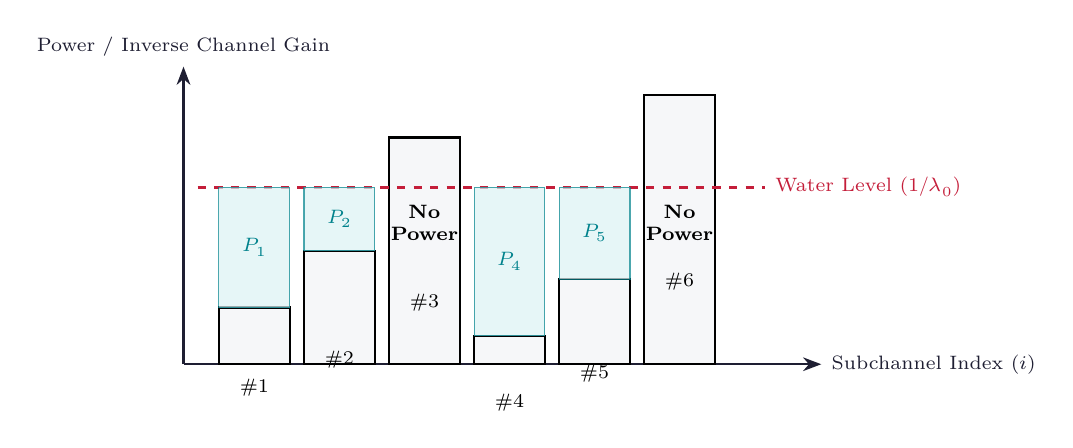
\begin{tikzpicture}[scale=0.9, every node/.style={font=\scriptsize}]
  % Draw axes
  \draw[arrow] (0,0) -- (9,0) node[right] {Subchannel Index ($i$)};
  \draw[arrow] (0,0) -- (0,4.2) node[above] {Power / Inverse Channel Gain};

  % Subchannel boxes (representing inverse gains N_0 * \Delta f / g_i)
  % Subchannel 1 (good gain, low inverse)
  \draw[thick, fill=mygray] (0.5, 0) rectangle (1.5, 0.8) node[midway, below=12pt] {\#1};
  % Subchannel 2 (moderate)
  \draw[thick, fill=mygray] (1.7, 0) rectangle (2.7, 1.6) node[midway, below=12pt] {\#2};
  % Subchannel 3 (poor, high inverse)
  \draw[thick, fill=mygray] (2.9, 0) rectangle (3.9, 3.2) node[midway, below=12pt] {\#3};
  % Subchannel 4 (excellent, lowest inverse)
  \draw[thick, fill=mygray] (4.1, 0) rectangle (5.1, 0.4) node[midway, below=12pt] {\#4};
  % Subchannel 5 (moderate)
  \draw[thick, fill=mygray] (5.3, 0) rectangle (6.3, 1.2) node[midway, below=12pt] {\#5};
  % Subchannel 6 (very bad, above water level)
  \draw[thick, fill=mygray] (6.5, 0) rectangle (7.5, 3.8) node[midway, below=12pt] {\#6};

  % Water Level line
  \draw[dashed, color=myred, line width=1.1pt] (0.2, 2.5) -- (8.2, 2.5) node[right, color=myred] {Water Level ($1/\lambda_0$)};

  % Allocated Power (Water) filling the bins up to the water level
  \fill[draw=myteal, fill=hdrteal, opacity=0.7] (0.5, 0.8) rectangle (1.5, 2.5);
  \node at (1, 1.65) {\color{myteal}\textbf{$P_1$}};
  
  \fill[draw=myteal, fill=hdrteal, opacity=0.7] (1.7, 1.6) rectangle (2.7, 2.5);
  \node at (2.2, 2.05) {\color{myteal}\textbf{$P_2$}};

  \fill[draw=myteal, fill=hdrteal, opacity=0.7] (4.1, 0.4) rectangle (5.1, 2.5);
  \node at (4.6, 1.45) {\color{myteal}\textbf{$P_4$}};

  \fill[draw=myteal, fill=hdrteal, opacity=0.7] (5.3, 1.2) rectangle (6.3, 2.5);
  \node at (5.8, 1.85) {\color{myteal}\textbf{$P_5$}};

  % Label for unallocated bin #3 and #6
  \node[align=center] at (3.4, 2.0) {\textbf{No}\\\textbf{Power}};
  \node[align=center] at (7.0, 2.0) {\textbf{No}\\\textbf{Power}};
\end{tikzpicture}
\end{tcolorbox}

% ===============================================================================
\section{Antennas for Mobile Terminals}
% ===============================================================================

Mobile terminal antennas must be compact, lightweight, and low-profile to fit within handheld devices while maintaining high radiation efficiency over multiple operating bands.

\subsection{Monopole Antennas}
A monopole antenna consists of a straight rod-shaped conductor mounted perpendicularly over a conducting ground plane.
\begin{itemize}[leftmargin=*, itemsep=3pt]
  \item \textbf{Working Principle:} When fed at its base, the antenna forms a resonant structure. By electromagnetic imaging theory, the conducting ground plane creates a virtual image of the monopole, causing it to behave like a half-wave ($\lambda/2$) dipole.
  \item \textbf{Length:} The standard physical length is a quarter-wavelength ($\lambda/4$).
  \item \textbf{Radiation Pattern:} Omnidirectional in the azimuth plane (horizontal), with a toroidal (donut-shaped) pattern in 3D.
  \item \textbf{Limitations:} Its vertical protrusion makes it unsuitable for modern, ultra-thin smartphones.
\end{itemize}

\subsection{Planar Inverted-F Antenna (PIFA)}
The PIFA is the dominant antenna technology for modern smartphones. It is derived from a conventional rectangular patch antenna by shorting the radiating patch to the ground plane at one end.

\begin{tcolorbox}[defbox]
\textbf{Planar Inverted-F Antenna (PIFA):} A low-profile, space-saving antenna consisting of a rectangular radiating patch suspended parallel to a ground plane, fed by a coaxial probe, and shorted to the ground plane at one edge using a shorting plate or pin. The shorting pin reduces the resonant length of the patch from $\lambda/2$ to $\lambda/4$.
\end{tcolorbox}

\begin{itemize}[leftmargin=*, itemsep=2.5pt]
  \item \textbf{Geometry:} The feed point is placed near the shorting pin. Adjusting the distance between the feed point and the shorting pin controls the input impedance, allowing easy matching to $50\,\Omega$ without external components.
  \item \textbf{Resonant Frequency Formula:} The approximate resonant frequency for a rectangular PIFA is:
    \begin{equation}
      f_r \approx \frac{c}{4(W + L)}
    \end{equation}
    Where $L$ and $W$ are the length and width of the radiating patch, and $c$ is the speed of light.
  \item \textbf{Advantages:} Ultra-low profile, easy to embed within device casings, reduced radiation toward the user's head (due to the shielding effect of the ground plane), and support for multi-band operation by slotting the patch.
\end{itemize}

\begin{tcolorbox}[tikzbox, title={Planar Inverted-F Antenna (PIFA) Structure}]
\centering
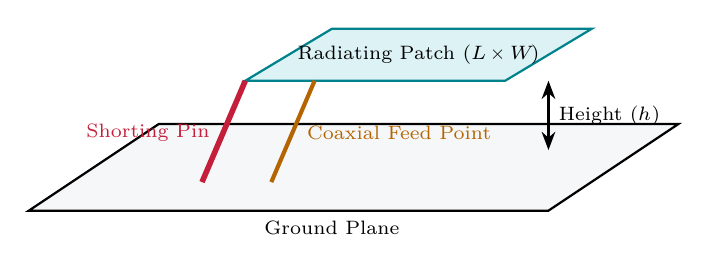
\begin{tikzpicture}[scale=1.1, every node/.style={font=\scriptsize}]
  % Draw Ground Plane (Base)
  \draw[thick, fill=mygray] (0,0) -- (6,0) -- (7.5,1) -- (1.5,1) -- cycle;
  \node[below] at (3.5,0) {Ground Plane};

  % Draw Radiating Patch (Suspended)
  \draw[thick, fill=hdrteal, draw=myteal] (2.5,1.5) -- (5.5,1.5) -- (6.5,2.1) -- (3.5,2.1) -- cycle;
  \node at (4.5, 1.8) {Radiating Patch ($L \times W$)};

  % Draw Shorting Wall/Pin
  \draw[line width=2pt, color=myred] (2.5,1.5) -- (2.0, 0.33);
  \node[left, color=myred] at (2.2, 0.9) {Shorting Pin};

  % Draw Feed Pin
  \draw[line width=1.5pt, color=myamber] (3.3,1.5) -- (2.8, 0.33);
  \node[right, color=myamber] at (3.1, 0.9) {Coaxial Feed Point};

  % Height indication
  \draw[Stealth-Stealth, thick] (6.0, 1.5) -- (6.0, 0.7) node[midway, right] {Height ($h$)};
\end{tikzpicture}
\end{tcolorbox}

% ===============================================================================
\section{Base Station Antennas and Arrays}
% ===============================================================================

Base station antennas must handle high RF power, shape radiation beams to cover specific geographic sectors, and dynamically adapt to user distribution.

\subsection{Omnidirectional vs. Sectorized Antennas}
\begin{itemize}[leftmargin=*, itemsep=3.5pt]
  \item \textbf{Omnidirectional Antennas:} Radiate power equally in all horizontal directions. Used in low-density rural areas or microcells with central base stations.
  \item \textbf{Sectorized Antennas:} Use directional antennas (typically panel antennas containing array dipoles) to concentrate radiation into a specific sector.
    \begin{itemize}[leftmargin=*, itemsep=2pt, topsep=2pt]
      \item \textbf{3-Sector Configuration:} 3 antennas, each covering a $120^\circ$ beamwidth (half-power beamwidth - HPBW).
      \item \textbf{6-Sector Configuration:} 6 antennas, each covering a $60^\circ$ beamwidth. Reduces co-channel interference, boosting network capacity.
    \end{itemize}
\end{itemize}

\begin{tcolorbox}[tikzbox, title={Base Station Sectorization Patterns}]
\centering
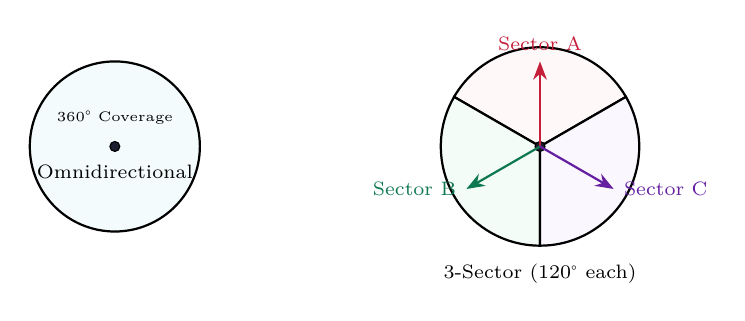
\begin{tikzpicture}[scale=0.9, every node/.style={font=\scriptsize}]
  % Omnidirectional cell (Circle)
  \draw[thick, fill=hdrteal!30] (-3,0) circle (1.2cm);
  \draw[fill=mydark] (-3,0) circle (2pt);
  \node[below=3pt] at (-3,0) {Omnidirectional};
  \node[font=\tiny] at (-3, 0.4) {360$^\circ$ Coverage};

  % Sectorized cell (3 Sectors of 120 degrees)
  \begin{scope}[shift={(3,0)}]
    \draw[thick, fill=hdrred!30] (0,0) -- (30:1.4) arc (30:150:1.4) -- cycle;
    \draw[thick, fill=hdrgreen!30] (0,0) -- (150:1.4) arc (150:270:1.4) -- cycle;
    \draw[thick, fill=hdrpurple!30] (0,0) -- (270:1.4) arc (270:390:1.4) -- cycle;
    \draw[fill=mydark] (0,0) circle (2pt);
    \node[below=3pt] at (0,-1.4) {3-Sector ($120^\circ$ each)};
    \draw[arrow, redarrow] (0,0) -- (90:1.2) node[above] {Sector A};
    \draw[arrow, color=mygreen] (0,0) -- (210:1.2) node[left] {Sector B};
    \draw[arrow, color=mypurple] (0,0) -- (330:1.2) node[right] {Sector C};
  \end{scope}
\end{tikzpicture}
\end{tcolorbox}

\subsection{Smart Antennas}
Smart antennas combine multiple antenna elements with digital signal processing to dynamically optimize the radiation pattern:
\begin{enumerate}[label=\textbf{\arabic*.}, leftmargin=*, itemsep=3.5pt]
  \item \textbf{Switched-Beam Antennas:} Feature a collection of fixed, directional beams. The system detects the user's signal strength and switches to the beam that provides the best alignment. It is simple but cannot track users continuously.
  \item \textbf{Adaptive Array Antennas:} Continuously adjust amplitude and phase weights (beamforming) to dynamically steer the main lobe of the antenna pattern toward the desired user while placing nulls in the direction of interferers.
\end{enumerate}

\subsection{Antenna Arrays}
An antenna array is a spatial arrangement of multiple antenna elements (usually dipoles or patches) fed with controlled phase and amplitude shifts:
\begin{itemize}[leftmargin=*, itemsep=3pt]
  \item \textbf{Array Factor ($AF$):} For a linear array of $M$ elements spaced at distance $d$:
    \begin{equation}
      AF(\theta) = \sum_{m=0}^{M-1} a_m e^{j m (k d \cos\theta + \beta)}
    \end{equation}
    Where $a_m$ is the amplitude weight, $k = 2\pi/\lambda$ is the wave number, $\beta$ is the progressive phase shift, and $\theta$ is the angle relative to the array axis.
  \item By adjusting $\beta$, the main beam can be steered electronically (\textbf{phased arrays}) without physically moving the antenna.
\end{itemize}

% ===============================================================================
% MANDATORY QUICK REVISION PAGE
% ===============================================================================
\newpage
\begin{center}
  {\large\bfseries\color{myred} Quick Revision --- Module III}\\[3pt]
  {\small\color{mydark} Channel Capacity and Mobile Antennas $|$ PE-EC701C}
\end{center}
\noindent{\color{myred}\rule{\linewidth}{1.2pt}}
\vspace{4pt}

\begin{tcolorbox}[formulabox, title={\textbf{Key Formulas at a Glance}}]
\renewcommand{\arraystretch}{1.3}
\begin{tabularx}{\linewidth}{B{5.5cm} X}
AWGN Channel Capacity & $C = B \log_2(1 + \text{SNR})$ \\
Ergodic Capacity (CSIR only) & $C = B \cdot \mathbb{E}\left[ \log_2(1 + \gamma) \right]$ \\
Water-Filling Power Allocation & $P_i = \left( \frac{1}{\lambda_0} - \frac{N_0 \Delta f}{g_i} \right)^{\!+}$ \quad ($\sum P_i = P_{\text{total}}$) \\
Outage Probability & $P_{\text{out}} = P(C(\gamma) < R)$ \\
PIFA Resonant Frequency & $f_r \approx \frac{c}{4(W + L)}$ \\
Monopole Resonant Length & $L \approx \frac{\lambda}{4}$ \\
Array Factor (Linear Array) & $AF(\theta) = \sum_{m=0}^{M-1} a_m e^{j m (k d \cos\theta + \beta)}$
\end{tabularx}
\end{tcolorbox}

\begin{tcolorbox}[defbox, title={\textbf{One-Line Definitions}}]
\begin{itemize}[leftmargin=*, itemsep=2.5pt, topsep=0pt]
  \item \textbf{Ergodic Capacity:} The long-term average transmission rate supported by a fast-fading channel.
  \item \textbf{Outage Capacity:} The maximum constant rate supported by a channel with a given outage probability threshold $\epsilon$.
  \item \textbf{Water-Filling:} An optimal power allocation strategy that prioritizes channels with high gains (low noise).
  \item \textbf{PIFA:} Planar Inverted-F Antenna, a compact, low-profile internal antenna used in mobile phones.
  \item \textbf{Monopole Antenna:} A resonant vertical rod antenna fed above a conducting ground plane.
  \item \textbf{Adaptive Array:} An antenna array that dynamically steers its beam toward the user and places nulls toward interferers.
  \item \textbf{Beamforming:} Shifting the phase and amplitude of array elements to create constructive interference in a desired direction.
\end{itemize}
\end{tcolorbox}

\begin{tcolorbox}[exambox, title={\textbf{Frequently Asked / Viva Questions}}]
\begin{enumerate}[topsep=0pt, label=\textbf{Q\arabic*.}, itemsep=5pt]
  \item \Q{Explain the physical meaning of the water-filling algorithm.}
    It mimics pouring a fixed volume of water (representing total power) into a vessel with an uneven bottom (representing inverse channel gains). The water fills the deepest valleys first, allocating more power to clean subchannels and no power to noisy ones.
  \item \Q{Why does a PIFA have a resonant length of $\lambda/4$ while a patch antenna requires $\lambda/2$?}
    Adding a shorting pin at the zero-electric-field boundary of a patch antenna enforces a short circuit. This changes the boundary condition, allowing the patch to resonate at a quarter-wavelength instead of a half-wavelength.
  \item \Q{Compare ergodic capacity and outage capacity.}
    Ergodic capacity represents the average rate supported over time in fast-fading channels. Outage capacity is used in slow-fading channels, representing the rate that can be guaranteed for $(1-\epsilon)\%$ of the time.
  \item \Q{What are the functions of the shorting pin and feed point in a PIFA?}
    The shorting pin forces a zero-voltage boundary condition, reducing the required physical size. Placing the feed point near the shorting pin allows the input impedance to be matched to $50\,\Omega$.
  \item \Q{Why are omnidirectional antennas not preferred at base stations in dense urban areas?}
    Omnidirectional antennas radiate power in all directions, causing high co-channel interference to adjacent cells. Sectorized antennas focus radiation, reducing co-channel interference.
  \item \Q{What is the difference between a switched-beam antenna and an adaptive array?}
    A switched-beam antenna switches between pre-configured, fixed directional beams. An adaptive array continuously calculates optimal weights to steer the main beam and nulls in real-time.
  \item \Q{What is the purpose of using antenna arrays at base stations?}
    To increase antenna gain, steer the radiation beam electronically (phased arrays), and enable spatial division multiple access (SDMA) and MIMO.
  \item \Q{State the resonant frequency approximation formula for a PIFA.}
    $f_r \approx \frac{c}{4(W+L)}$, where $L$ and $W$ are the length and width of the radiating plate, and $c$ is the velocity of light.
  \item \Q{Why is a monopole antenna modeled as a dipole over a ground plane?}
    According to the electromagnetic image theory, a conducting ground plane creates a virtual image of the vertical monopole below the plane, acting as the second half of a dipole.
  \item \Q{What is the impact of placing the feed point close to the shorting pin in PIFA?}
    As the feed point moves closer to the shorting pin, the input impedance decreases toward zero. This allows the input impedance to be matched to $50\,\Omega$.
  \item \Q{Explain how electronic beam steering is achieved in antenna arrays.}
    By introducing a progressive phase shift $\beta$ between adjacent antenna elements. This shifts the direction where the signals add constructively, steering the beam without physical rotation.
  \item \Q{Under what conditions does the water-filling algorithm allocate zero power to a subchannel?}
    When the subchannel's normalized noise-to-gain ratio ($N_0 \Delta f / g_i$) is higher than the calculated water-level threshold ($1/\lambda_0$).
\end{enumerate}
\tcbset{colbacktitle=myteal, coltitle=white}
\end{tcolorbox}

\begin{tcolorbox}[tikzbox, title={Comparison of Monopole and PIFA Antennas}]
\renewcommand{\arraystretch}{1.4}
\par\noindent
{\renewcommand{\arraystretch}{1.55}%
\begin{tabularx}{\linewidth}{|B{3.0cm}|Y|Y|}
\hline
\textbf{Parameter} & \textbf{\color{myteal}Monopole Antenna} & \textbf{\color{myred}Planar Inverted-F (PIFA)} \\[4pt]
\hline
\textbf{Structure} & Simple vertical rod over a ground plane. & Flat rectangular patch parallel to a ground plane with a shorting pin. \\[4pt]
\hline
\textbf{Resonant Length} & $\lambda/4$ (vertical height). & $\approx \lambda/4$ (sum of length and width, $L+W$). \\[4pt]
\hline
\textbf{Profile} & High profile (protruding structure). & Low profile, easily embedded inside devices. \\[4pt]
\hline
\textbf{SAR (Radiation towards head)} & High (radiates symmetrically around the rod). & Low (ground plane acts as an electromagnetic shield). \\[4pt]
\hline
\end{tabularx}
}
\tcbset{colbacktitle=myteal, coltitle=white}
\end{tcolorbox}

\end{document}
